\subsection{Universities: Visions of
Utopia}\label{universities-visions-of-utopia}

If the university campus lived up to its potential it could be a true
paradise: essentially a giant garden filled with buildings for studying
and creating knowledge. Amazing! They are usually situated on some of
the best land to be found anywhere, have great access to everything
needed in life, and have dense urban style housing in a pastoral
environment which allows for a simple, car free life.

University campuses are often physically spectacular. They often have
some of the greatest examples of art and architecture of available both
used in their construction and lovingly maintained for in some cases
hundreds of years. It is typical for them to have wooded areas owned by
the university, as well as often running water and in many cases access
to very large bodies of water. University campuses are often more self
contained than most institutions, creating their own power and managing
their own utilities, and having a fair amount of autonomy from local
government.

\subsection{Brief History of the
University}\label{brief-history-of-the-university}

Where did the universities come from?

University as a challenge to secular corporate rule.

Looking up sources at UAA library.

The universities of Europe, 1100-1914 : a history is at LA627.R82 1984

This needs extensive library research.

\subsection{Undergraduate Education: Broken
Promises}\label{undergraduate-education-broken-promises}

The college education has become a key element in the great lie of the
American middle class dream. It is also a major factor in the older
generation destroying the opportunities they had for the younger
generation.

\subsection{Science Grad School: The Ponzi
Scheme}\label{science-grad-school-the-ponzi-scheme}

You don't have to go to graduate school to see how much it resembles a
pyramid scam. Suppose any one professor has about five graduate students
at a time, each of whom takes about five years to graduate with a PhD.
If a professor does this for 30 years, they will create on average one
PhD per year or 30 PhD's total. Now suppose all those PhD's find jobs
similar to what their advisor has. This is possible only if the size of
the field increases by 30 times in 30 years. Very crudely this
corresponds to about 12\% per year. Given the expansion of the physical
sciences and their satellites in the years during and directly after
World War II, building a scheme like this in those years actually made
some sense. However, those days are decades behind us, and now as
research budgets shrink and schools, companies, and government agencies
are systematically destroyed by politics, this math looks much more like
a pyramid scam than a response to society's needs.

As a grad student you will \emph{probably} never get the job you're
supposedly being trained for. But you will dedicate 5-7 years of your
life to helping someone who \emph{did} get that job to continue to climb
the academic ladder. The people at the bottom of the academic pyramid
spend their lives working to help the people at the top, and then are
mostly cast aside.

The tenure clock then puts yet another opportunity for exploitation in
the career path, making yet another way for people now well into middle
age to work long hours for more years to build up an academy that they
might then be cast out of.

\subsection{Hollowing Out of the
Academy}\label{hollowing-out-of-the-academy}

There are many factors that have contributed to the downfall of the
university system over the last few years. I would argue that since
Ronald Reagan was elected president of the United States in 1980 there
has been a coordinated ideological war against all culture that might
exist outside of the profit system, and that universities have felt the
brunt of this particularly hard.

A robust, healthy, independent, and publicly supported university system
could provide a real balance against mainstream corporate power if it
existed. It is therefore strategically important for the lords of global
corporate rule that they be as controlled as possible by corporations
and the central government so that they cannot exercise a check on those
forms of power.

\subsection{Intellectual Property}\label{intellectual-property}

\subsection{Potential Paradises}\label{potential-paradises}

\subsection{University Occupations, Phase
2}\label{university-occupations-phase-2}

Any history of any radical movement will inevitably involve student
occupations. Students typically take over some space on campus, keep the
land from the cops, and carry out various protest actions or teach ins
over some number of days or maybe weeks. In some cases they stand down
after actually getting some demands met by the administration.

\subsection{Case Study: Yale
University}\label{case-study-yale-university}

\begin{itemize}
\tightlist
\item
  How much land owned?
\item
  How much is arable?
\item
  How much is already zoned for ag?
\item
  What water resrouces are there?
\item
  number of staff, students, alumni, faculty
\item
  How many people could Yale support?
\item
  Holdings outside New Haven
\item
  Yale Singapore
\item
  Repurposing the Endowment, total divestment from capitalism
\item
  political and legal process of re-writing the charter of the school,
  changing governance
\end{itemize}

yale history:
https://www.worldcat.org/title/yale-university/oclc/40331263\&referer=brief\_results

yale land holdings:

\url{http://sustainability.yale.edu/planning-progress/areas-focus/landscape}

charter:
\url{http://www.yale.edu/sites/default/files/files/University-Charter.pdf}

\subsection{Case Study: University of
Paris(Sorbonne)}\label{case-study-university-of-parissorbonne}

\begin{figure}[htbp]
\centering
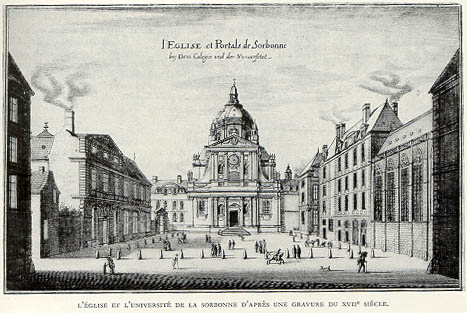
\includegraphics{images/Sorbonne_17thc.jpg}
\caption{The Sorbonne}
\end{figure}

\url{https://en.wikipedia.org/wiki/University_of_Paris}

\url{https://en.wikipedia.org/wiki/University_of_Paris_strike_of_1229}

\subsection{Case Study: Roosevelt
Island}\label{case-study-roosevelt-island}

\url{https://en.wikipedia.org/wiki/Cornell_Tech}

\subsubsection{this chapter should have a section with a detailed
example}\label{this-chapter-should-have-a-section-with-a-detailed-example}

maps, tables, really dig in and figure out the strategy and tactics that
could be used, maybe have multiple examples, small liberal arts, huge
public school, elite private school, community college in a big city

\subsubsection{The Universities are a
Disaster}\label{the-universities-are-a-disaster}

\begin{itemize}
\item
  Academia as pyramid scam
\item
  Academia as tool of the military industrial State
\item
  Academia as a marketing tool for the banking cartel
\item
  Academia: where ideas go to die
\item
  Academia: it was here before capitalism and it will be here after
\item
  Has traditionally been a part of various religions and patriarchal
  systems connected with them
\end{itemize}

IP is key to how bad it is, academia after the re-occupation of the
campus all property will be banned from campus.

\subsubsection{But they're really useful to
us}\label{but-theyre-really-useful-to-us}

Back to basics: knowledge, teaching, philosophy, technology, culture,
books, land, food and energy

Universities must be Occupied and declared independent

This should be across disciplines and outside of the capitalist class
system, bringing in workers, locals, students, teachers, researchers and
everyone else involved. Seize the legal control of the corporation that
is the University, and you will have a power that States must respect.

Taking universities over can be a huge international beach head that
goes around all national borders.

Important reference:

Universities, Inc.

call number: 338.43378 WASHBURN

DPL description:

``Our federal and state tax dollars are going to fund higher education.
If corporations kick in a little more, should they be able to dictate
the research or own the discoveries?During the past two decades,
commercial forces have quietly transformed virtually every aspect of
academic life. Corporate funding of universities is growing and the
money comes with strings attached. In return for this funding,
universities and professors are acting more and more like for-profit
patent factories: university funds are shifting from the humanities and
the less profitable science departments into research labs, and the
skill of teaching is valued less and less. Slowly but surely,
universities are abandoning their traditional role as disinterested
sources of education, alternative perspectives, and wisdom.This growing
influence of corporations over universities affects more than just
today's college students (and their parents); it compromises the future
of all those whose careers depend on a university education, and all
those who will be employed, governed, or taught by the products of
American universities.''
